\documentclass[]{article}
\usepackage{lmodern}
\usepackage{amssymb,amsmath}
\usepackage{ifxetex,ifluatex}
\usepackage{fixltx2e} % provides \textsubscript
\ifnum 0\ifxetex 1\fi\ifluatex 1\fi=0 % if pdftex
  \usepackage[T1]{fontenc}
  \usepackage[utf8]{inputenc}
\else % if luatex or xelatex
  \ifxetex
    \usepackage{mathspec}
  \else
    \usepackage{fontspec}
  \fi
  \defaultfontfeatures{Ligatures=TeX,Scale=MatchLowercase}
\fi
% use upquote if available, for straight quotes in verbatim environments
\IfFileExists{upquote.sty}{\usepackage{upquote}}{}
% use microtype if available
\IfFileExists{microtype.sty}{%
\usepackage{microtype}
\UseMicrotypeSet[protrusion]{basicmath} % disable protrusion for tt fonts
}{}
\usepackage[margin=1in]{geometry}
\usepackage{hyperref}
\hypersetup{unicode=true,
            pdftitle={Notes},
            pdfborder={0 0 0},
            breaklinks=true}
\urlstyle{same}  % don't use monospace font for urls
\usepackage{graphicx,grffile}
\makeatletter
\def\maxwidth{\ifdim\Gin@nat@width>\linewidth\linewidth\else\Gin@nat@width\fi}
\def\maxheight{\ifdim\Gin@nat@height>\textheight\textheight\else\Gin@nat@height\fi}
\makeatother
% Scale images if necessary, so that they will not overflow the page
% margins by default, and it is still possible to overwrite the defaults
% using explicit options in \includegraphics[width, height, ...]{}
\setkeys{Gin}{width=\maxwidth,height=\maxheight,keepaspectratio}
\IfFileExists{parskip.sty}{%
\usepackage{parskip}
}{% else
\setlength{\parindent}{0pt}
\setlength{\parskip}{6pt plus 2pt minus 1pt}
}
\setlength{\emergencystretch}{3em}  % prevent overfull lines
\providecommand{\tightlist}{%
  \setlength{\itemsep}{0pt}\setlength{\parskip}{0pt}}
\setcounter{secnumdepth}{0}
% Redefines (sub)paragraphs to behave more like sections
\ifx\paragraph\undefined\else
\let\oldparagraph\paragraph
\renewcommand{\paragraph}[1]{\oldparagraph{#1}\mbox{}}
\fi
\ifx\subparagraph\undefined\else
\let\oldsubparagraph\subparagraph
\renewcommand{\subparagraph}[1]{\oldsubparagraph{#1}\mbox{}}
\fi

%%% Use protect on footnotes to avoid problems with footnotes in titles
\let\rmarkdownfootnote\footnote%
\def\footnote{\protect\rmarkdownfootnote}

%%% Change title format to be more compact
\usepackage{titling}

% Create subtitle command for use in maketitle
\providecommand{\subtitle}[1]{
  \posttitle{
    \begin{center}\large#1\end{center}
    }
}

\setlength{\droptitle}{-2em}

  \title{Notes}
    \pretitle{\vspace{\droptitle}\centering\huge}
  \posttitle{\par}
    \author{}
    \preauthor{}\postauthor{}
    \date{}
    \predate{}\postdate{}
  

\begin{document}
\maketitle

\hypertarget{packrat}{%
\subsection{packrat}\label{packrat}}

Reproducible package manamement for R. Makes your R projects
reproducible by making them

\begin{itemize}
\tightlist
\item
  \textbf{isolated}: installing other packages won't break your project
\item
  \textbf{portable}: easy to share, even cross platform
\item
  \textbf{reproducible}: because it records the exact versions of the
  packages your project depends on
\end{itemize}

Each project has its own package library.

Funny story: so I've known about packrat for a few years now. I've known
what it does, and it made all the sense in the world. And yet I didn't
use it. God knows what my problem is, but it was only last month, when I
bought a new laptop, installed a new and different OS than my previous
one and wanted to start working on a project I was working on in the
spring, when it suddenly didn't work anymore. It was a big project with
dozens of interconnected files and several dozen packages, and it was
now broken. Now, I had already returned my old laptop to my employer so
I had no way of recreating the package environment that I had there. And
no easy way of figuring out which of the packages was the offending
package that had been updated in the meantime.

And it made me realise how incredibly lucky I had been that the
client---this was a consulting gig---the client was able to run the code
on their systems without any problems, presumably because theey had the
same outdated libraries installed as I had had on my old laptop. I was
terribly lucky, but I learned my lesson anyway. So from then on I use
packrat, actually preparing this talk was the first time I used it on a
new project.

But I wanted to bring up this story also to demonstrate that it is often
a slog, this reproducibility stuff. It's upfront work, and it's easy to
put it off. Although in the end it turned out that packrat is
ridiculously easy to setup, it is literally just one line of code, and
if you're initializing it on an existing large project you'll have time
to make yourself a quick cup of tea while it creates the snapshot of the
working library environment, but I was quite embarassed once I realised
I could have been doing this for years.. Instead I had to first have it
go wrong and have the code break, before I came to my senses and started
using this tool. It's normal, it's human. But it's also stupid. So don't
be stupid like I was, it's a lot less painful to get on the
reproduciblility bandwagon of your own accord than learning the hard
way.

\hypertarget{how-to-cite-software}{%
\subsection{how to cite software}\label{how-to-cite-software}}

(Jackson, n.d.)

\begin{itemize}
\tightlist
\item
  Which software should be cited?

  \begin{itemize}
  \tightlist
  \item
    Critical and/or novel contribution.
  \item
    sometimes the licence requires you cite it
  \end{itemize}
\item
  How should it be cited?

  \begin{itemize}
  \tightlist
  \item
    find your citation style's examples
  \item
    do not use cite associated papers instead!
  \item
    if there is a DOI, use it!
  \end{itemize}
\item
  Where should you cite it?

  \begin{itemize}
  \tightlist
  \item
    if cannot cite in references then footnotes are second best option
  \item
    or methods section or appendix or supplementary materials, as long
    as it is there!
  \end{itemize}
\end{itemize}

One way or another it is highly likely that software played an important
role in you producing your research. This contribution should be
acknowledged. Now this doesn't mean you have to make sure everyone knows
you used Microsoft Word to write your paper, a good rule of thumb is to
ask yourself if the software contributed critically to your research
and/or if it provided something novel. This is the recommendation of the
British Software sustainability insititute. If this feels a bit
ambiguous, I would suggest you err on the side of citing rather than
not.

For example you might think it silly to acknowledge that you used
Microsoft Excel to do your analysis, but that is only if you thing it
the software is faultless and your analysis would have produced the
exact same results in any spreadhseet programme. But that may not be
true. Excel--not to pick on any specific programme--but it has a bunch
of quirks that are specific to it, you might even call them bugs. And
they could very well affect your analysis, which counts as having a
critical contribtution.

For example Excel treats 1900 as a leap year. This is due to some
historical reasons, to make it compatible with IBM's Lotus-1-2-3 if
you're old enough to remember it. Anyway, Microsoft aknowledges that
this means ``The WEEKDAY function returns incorrect values for dates
before March 1, 1900. Because most users do not use dates before March
1, 1900, this problem is rare.''

Well, perhaps most users don't but I'm sure with this group of people
that is not unheard of\ldots{} There are other bugs as well, for example
the 2007 version had a bug that incorrectly reported the product of 12
pairs of numbers. I think 77.1 times 850 was reported as 100,000 instead
of correctly as 65 thousand and something. It would be incredibly
unlikely that that error affected your research, but if it did, you can
bet that it's impact would be quite critical, so again, I would
definitely go so far as to cite even the spreadsheet programme you used.

But more generally you should cite any software that impacts upon the
results, includes numerical modelling or simulations, any algorithmic
evaluations or research using software that does some form of automated
analysis e.g.~image analysis or optical character recognition.

Sometimes the decision is made for you, because the licence for the
software, that you have of course carefully read, so you know this, but
sometimes the licence explicitly requires you cite it.

How should software be cited?

All the main citation styles have examples of how to cite software. For
example MLA suggests:

``SPSS Student Version 11.0.'' Prentice Hall, 2001.

And you should be able to look up examples for your prefered style.
Whatever you choose though, make sure you include the version of the
software. The idea is for you to be transparent about how your results
were produced and allow someone else to replicate them, and software
versions could play a role here.

Additionally most software developers will have a suggested citation
format.

Sometimes it seems more straightforward to cite the associated paper for
a programme instead of the software itself. It fits the format we're
used to, I guess it's always nicer to cite a person than an institution
or company. You should avoid doing that. Always cite the software
explicitly. If the associated paper was substatnively useful in your
analysis, then by all means cite it as well, additionally, but not
instead.

Several reasons for this: not all software has associated journal
articles. Also an article is not specific to the version you were using,
so does not serve to enhance reproducibility in that way.

Publishers and reviewers might take issue with the citing of software,
however that sort of attitide is hopefully becoming a thing of the past.
If you were to receive pushback the alternative is always to include the
citation information in a footnote or otherwise stated in the methods
section. From the point of view of reproducibility, the important thing
is the information is accessible to the reader. However from the point
of view of the authors, especially if they have mandated citation in the
licence, that may be too little.

If the software you are using has a DOI, then use it! Use it even at the
expense of a url. Because DOIs are perseistent and urls are not. If you
cite the DOI in its url form with the resolver service url as its
prefix, for example like this \url{http://dx.doi.org/NNNN,then} it will
work like a link and lead to the source, even if it has moved in the
meantime.

If there is no DOI, use urls, even though MLA recommends against it
(becuase of breakage). It is still better

Examples Software purchased off-the-shelf:

ProductName. Version. ReleaseDate. Publisher. Location.

SuperScience. 1.2. December 2012. ResearchSoftware. Edinburgh, UK.

Software downloaded from the web:

ProductName. Version. ReleaseDate. Publisher. Location. DOIorURL.
DownloadDate.

OGSA-DAI REST. 4.2.1. December 2012. OGSA-DAI Project.
\url{http://sourceforge.net/projects/ogsa-dai}. 27/04/2012.

UltimateFFT. 2.4. December 2012. Fred Bloggs, EPCC, The University of
Edinburgh, UK. \url{http://www.epcc.ed.ac.uk/ultimate-fft}. 27/04/2012.

C implementation of Wu's color quantizer. 2. 1991. Xiaolin Wu,
Department of Electrical \& Computer Engineering, McMaster University,
Hamilton, Ontario. \url{http://www.ece.mcmaster.ca/~xwu/cq.c}.
27/04/2012.

Software checked-out from a public repository:

ProductName. Publisher. URL. CheckoutDate.
RepositorySpecificCheckoutInformation.

OGSA-DAI REST. OGSA-DAI Project.
\url{http://sourceforge.net/projects/ogsa-dai}. 27/04/2012. Check-out:
ogsa-dai/branck/ogsadai4.1/, revision 1657.

Software provided by a researcher:

ProductName. Author. Location. ContactDetails. ReceivedDate.
BestFFTroutine ever file. Fred Bloggs, EPCC, The University of
Edinburgh, UK.
\href{mailto:Fred.bloggs@epcc.ed.ac.uk}{\nolinkurl{Fred.bloggs@epcc.ed.ac.uk}}.
27/04/2012. (Hong et al. 2015)

\hypertarget{additional-details}{%
\subsection{additional details}\label{additional-details}}

In addition to software there are other environmental variables that
should be explicitly stated if they affect the results: " This
information may include: operating system, specific packages,
sub-routines, queries, files, libraries, scripts, service end-points,
configurations, parameters or workflows" "this information should be
described in the body of your paper, in the methods section, footnotes,
acknowledgements or appendices.

\begin{figure}

\includegraphics[width=2000]{/home/mz/Dropbox/XtraWork/teaching/2019-07-rep-res-humanities-oxford//figures/final-doc} \caption{PhD: final.doc [http://phdcomics.com/comics/archive.php?comicid=1531]}\label{fig:phd}
\end{figure}

\hypertarget{style-guide}{%
\subsection{style guide}\label{style-guide}}

\begin{figure}
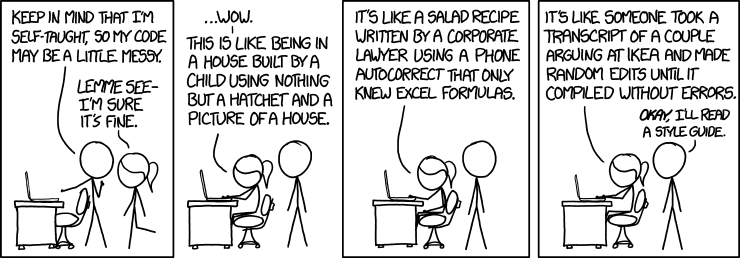
\includegraphics[width=1.1\linewidth]{/home/mz/Dropbox/XtraWork/teaching/2019-07-rep-res-humanities-oxford//figures/code_quality} \caption{[xkcd: Code Quality [https://xkcd.com/1513/]}\label{fig:xkcd}
\end{figure}

text

\hypertarget{references}{%
\section*{References}\label{references}}
\addcontentsline{toc}{section}{References}

\hypertarget{refs}{}
\leavevmode\hypertarget{ref-hong2015top}{}%
Hong, Neil P Chue, Tom Crick, Ian P Gent, Lars Kotthoff, and Kenji
Takeda. 2015. ``Top Tips to Make Your Research Irreproducible.''
\emph{arXiv Preprint arXiv:1504.00062}.

\leavevmode\hypertarget{ref-jacksonNodate}{}%
Jackson, Mike. n.d. ``How to Cite and Describe Software.'' Software
Sustainability Institute;
\url{https://software.ac.uk/how-cite-software}.


\end{document}
